\begin{pastexam}[label={px:ntust-108-ice-05}]{臺科大資工所 108 學年度 第 5 題}
（問答）

Given the preorder and inorder sequences of a binary tree as follows: (15\%)

\begin{tabular}{ll}
Preorder: & JIDHCBEFGA \\
Inorder: & HDIBCJFEGA
\end{tabular}

Assume that each character represents a node in the tree.
\begin{enumerate}[label=(\alph*)]
\item Please draw the corresponding binary tree. (10\%)
\item Please provide the postorder sequence of the tree. (5\%)
\end{enumerate}
\end{pastexam}

\begin{pastsoln}
答案：(a) 見下圖；(b) HDBCIFAGEJ。

前序加中序可以唯一決定一棵二元樹（資結書定理~7.4）。 做法（資結書虛擬碼~7.5）：前序的第一個是根；
在中序裡找到根，左邊是左子樹、右邊是右子樹；左子樹有幾個節點，前序裡根後面就切幾個給左子樹，
兩邊再遞迴。

\textbf{(a)} 逐層拆：
\begin{itemize}
\item 前序 JIDHCBEFGA、中序 HDIBC\,\textbf{J}\,FEGA：根 J。 左子樹中序 HDIBC（$5$ 個），前序取 J 後面
$5$ 個 IDHCB；右子樹中序 FEGA，前序 EFGA。
\item 左子樹：前序 IDHCB，根 I；中序 HD\,\textbf{I}\,BC。 左邊 HD（前序 DH），右邊 BC（前序 CB）。
\begin{itemize}
\item 前序 DH、中序 HD：根 D，H 在 D 左邊，是 D 的左子節點。
\item 前序 CB、中序 BC：根 C，B 在 C 左邊，是 C 的左子節點。
\end{itemize}
\item 右子樹：前序 EFGA，根 E；中序 F\,\textbf{E}\,GA。 左邊 F；右邊 GA（前序 GA）。
\begin{itemize}
\item 前序 GA、中序 GA：根 G，A 在 G 右邊，是 G 的右子節點。
\end{itemize}
\end{itemize}
\begin{center}
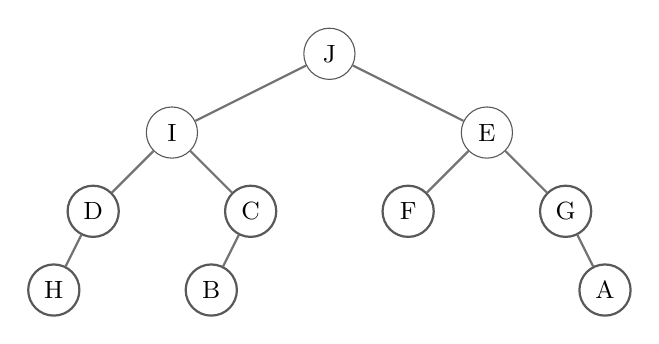
\begin{tikzpicture}[level distance=10mm,
  every node/.style={circle,draw=black!65,minimum size=6.5mm,inner sep=0pt,font=\small},
  edge from parent/.style={draw=black!55,thick},
  level 1/.style={sibling distance=40mm},
  level 2/.style={sibling distance=20mm},
  level 3/.style={sibling distance=10mm}]
\node {J}
  child {node {I}
    child {node {D}
      child {node {H}}
      child[missing]}
    child {node {C}
      child {node {B}}
      child[missing]}}
  child {node {E}
    child {node {F}}
    child {node {G}
      child[missing]
      child {node {A}}}};
\end{tikzpicture}
\end{center}
檢查：這棵樹的前序是 J I D H C B E F G A、中序是 H D I B C J F E G A，都和題目相同。

\textbf{(b)} 後序是「左、右、根」（資結書第~7.3~節）。 左子樹 I：先 D 的子樹（H、D），再 C 的子樹
（B、C），最後 I；右子樹 E：F，再 G 的子樹（A、G），最後 E；最後根 J：
\[
\text{H D B C I F A G E J}.
\]
\end{pastsoln}
